\section{Block Ciphers}\label{sec:Block_Ciphers}
\begin{definition}[Block Cipher]\label{def:Block_Cipher}
  A \emph{block cipher} encrypts a fixed-length block of plaintext bits $x$ to a fixed-length block of ciphertext $y$.
  This transformation is controlled by the secret key $K$, and is written $E_{K}(x) = y$.

  The secret key defines a fixed mapping of the plaintext block $x$ to the ciphertext block $y$.
  This can sometimes make block ciphers a form of \nameref{subsec:Simple_Substitution_Cipher}.

  Block ciphers are usually implemented with several \nameref{def:Round_Function}s, based on the \nameref{def:Round_Key}.
\end{definition}

\begin{definition}[Round Function]\label{def:Round_Function}
  \nameref{def:Block_Cipher}s are usually implemented as iterated ciphers, where a simple encryption function is iteratively applied for $N$ rounds.
  This is called a \emph{round function}.
  It is commonly denoted
  \begin{equation}\label{eq:Round_Function}
    h(w_{i-1}, k_{i})
  \end{equation}
  where
  \begin{itemize}[noitemsep]
  \item $i$ is the current round (current iteration).
  \item $w$ is the input plaintext block.
  \item $k$ is the \nameref{def:Round_Key} on the $i$th iteration.
  \item $h$ is the \nameref{def:Round_Function}.
  \end{itemize}

  These functions must also be invertible, namely,
  \begin{equation}\label{eq:Round_Function_Invertible}
    h^{-1} \bigl( h(w_{i-1}, k_{i}), k_{i} \bigr) = w_{i-1}
  \end{equation}

  \textbf{These functions must be efficient to compute, and be efficient to compute the inverse round function.}
\end{definition}

\begin{definition}[Round Key]\label{def:Round_Key}
  The \emph{round key} is derived from the key $K$.
  The way in which the round key is derived from $K$ is called the \emph{key schedule}.
\end{definition}

If we want to mathematically illustrate the implementation of a \nameref{def:Block_Cipher}'s encryption with a iterative cipher, it is defined as:
\begin{align*}
  w_{0} &= x \\
  w_{1} &= h(w_{0}, k_{1}) \\
  w_{2} &= h(w_{1}, k_{2}) \\
        &\vdots \\
  w_{N-1} &= h(w_{N-2}, k_{N-1}) \\
  w_{N} &= h(w_{N-1}, k_{N}) \\
\end{align*}
\begin{itemize}[noitemsep]
\item $x$ is the plaintext block.
\item $w_{i}$ are intermediate values in the implementation of the iteration.
\item $w_{N}$ is the final output from the cipher.
\item $h(w_{i-1}, k_{i})$ denotes the round function.
\item $k_{i}$ is the round key used in the $i$th round.
\end{itemize}

For the same iterative cipher, the decryption function $D_{K}(y)$ is just the application of the \nameref{def:Round_Key}s in reverse order.
\begin{align*}
  w_{N} &= y \\
  w_{N-1} &= h^{-1}(w_{N}, k_{N}) \\
  w_{N-2} &= h^{-1}(w_{N-1}, k_{N-2}) \\
        &\vdots \\
  w_{1} &= h^{-1}(w_{2}, k_{2}) \\
  w_{0} &= h^{-1}(w_{1}, k_{1}) = x \\
\end{align*}

\subsection{Examples of Iterated Ciphers}\label{subsec:Examples_Iterated_Ciphers}
\subsubsection{Feistel Ciphers/DES}\label{subsubsec:Feistel_Cipher_DES}
\begin{definition}[Feistel Cipher]\label{def:Feistel_Cipher}
  A \emph{Feistel cipher} is a type of iterated cipher that is easy to implement in both hardware and software.
  However, it is not safe to use anymore.

  An example of these is the DES encryption algorithm.

  The block being run through the \nameref{def:Round_Function} is split in half; a left and right half, denoted
  \begin{equation}\label{eq:Feistel_Cipher_Block}
    w_{i} = (L_{i}, R_{i})
  \end{equation}

  The \nameref{def:Round_Function} $h(L_{i-1}, R_{i-1}, k_{i})$ is implemented as
  \begin{equation}\label{eq:Feistel_Cipher_Round_Function_Encryption}
    \begin{aligned}
      L_{i} &= R_{i-1} \\
      R_{i} &= L_{i-1} \XOR f(R_{i-1}, k_{i})
    \end{aligned}
  \end{equation}
  where $f(R_{i-1}, k_{i})$ can be any function.

  The decryption function for the Feistel cipher is implemented as
  \begin{equation}\label{eq:Feistel_Cipher_Round_Function_Decryption}
    \begin{aligned}
      L_{i-1} &= R_{i} \XOR f(R_{i-1}, k_{i}) \\
      R_{i-1} &= L_{i}
    \end{aligned}
  \end{equation}
  and $(L_{0}, R_{0})$ gives back $x$.
\end{definition}

\subsubsection{SP Network}\label{subsubsec:SP_Network}
\begin{definition}[SP Network]\label{def:SP_Network}
  An \emph{SP network} is a iterated \nameref{def:Block_Cipher} that consists of a mix between substitutions (\emph{S}) (\nameref{subsec:Simple_Substitution_Cipher}s) and permutations (\emph{P}) or linear transformations (~\pageref{subsubsec:Transposition_Cipher}s).
  The \nameref{def:Round_Key} is added to the input to the \nameref{def:Round_Function} in a simple way ($\XOR$).

  An example of these is the AES (Advanced Encryption Scheme) cipher.
\end{definition}

\begin{definition}[S-Box]\label{def:S_Box}
  An \emph{S-Box} is the substitution portion of an \nameref{def:SP_Network}.
  They are usually taken over a small alphabet, and only have 4, 6, or 8 bits as input.
\end{definition}

\subsection{Modes of Operation}\label{subsec:Modes_of_Operation}
\begin{definition}[Mode of Operation]\label{def:Mode_of_Operation}
  A \emph{mode of operation} describes how to repeatedly apply a cipher's single-block operation to securely transform amounts of data larger than a block.
  This is helpful because, by themselves, \nameref{def:Block_Cipher}s can only encrypt/decrypt one block.
  To accomplish this, the plaintext is split up into blocks, and each block is encrypted.
  \begin{equation*}
    x_{1}, x_{2}, \ldots, x_{N}, x_{N+1}, \ldots
  \end{equation*}

  Let $X_{1} = (x_{1}, x_{2}, \ldots, x_{N})$ be the first block with length $N$.
  Let $X_{2} = (x_{N+1}, x_{N+2}, \ldots, x_{2N})$ be the second block, also with length $N$.
  The encryption is then done blockwise
  
  Most modes require a unique binary sequence, often called an \nameref{def:Initialization_Vector} (IV), for each encryption operation.

  There are 3 modes of operation that are discussed in this course:
  \begin{enumerate}[noitemsep]
  \item \nameref{subsubsec:Electronic_Codebook_Mode}
  \item \nameref{subsubsec:Cipher_Block_Chaining_Mode}
  \item \nameref{subsubsec:Counter_Mode}
  \end{enumerate}
\end{definition}

\begin{definition}[Initialization Vector]\label{def:Initialization_Vector}
  An \emph{initialization vector} (\emph{IV}) is a unique binary sequence that is used for each encryption operation.
  The IV has to be non-repeating and, for some modes, random as well.
\end{definition}

\subsubsection{Electronic Codebook (ECB) Mode}\label{subsubsec:Electronic_Codebook_Mode}
\begin{equation}\label{eq:Electronic_Codebook_Mode_Encryption}
  C_{I} = E_{K}(X_{i}) \:\: i=1, 2, \ldots
\end{equation}

The steps required to operate a block cipher in ECB mode are illustrated in \Crefrange{subfig:ECB_Mode_Steps_Encryption}{subfig:ECB_Mode_Steps_Decryption}.
\begin{figure}[ht!]
  \centering
  \begin{subfigure}[h!]{0.45\linewidth}
    \centering
    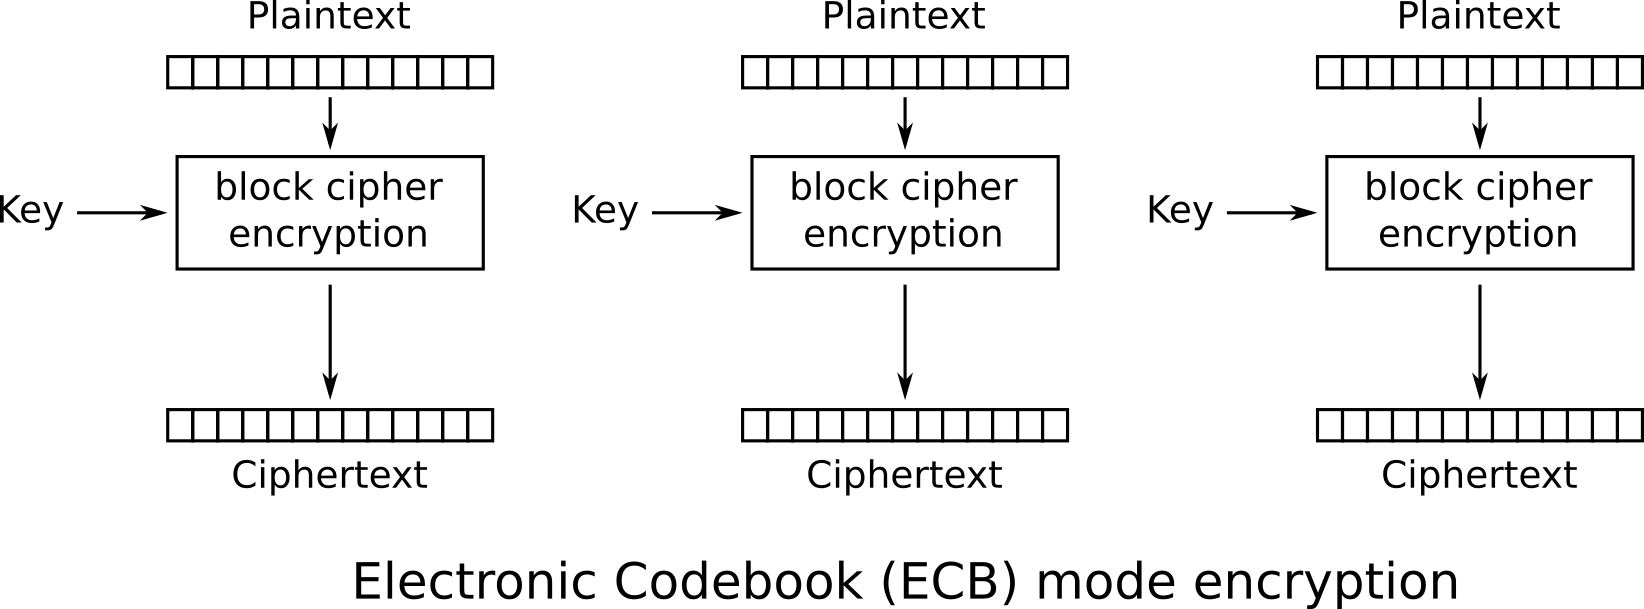
\includegraphics[scale=0.55]{./Drawings/EDIN01-Cryptography/ECB_Mode-Encryption.png}
    \caption{\nameref{subsubsec:Electronic_Codebook_Mode} Encryption Steps}
    \label{subfig:ECB_Mode_Steps_Encryption}
  \end{subfigure}
  \vline{}
  \begin{subfigure}[h!]{0.45\linewidth}
    \centering
    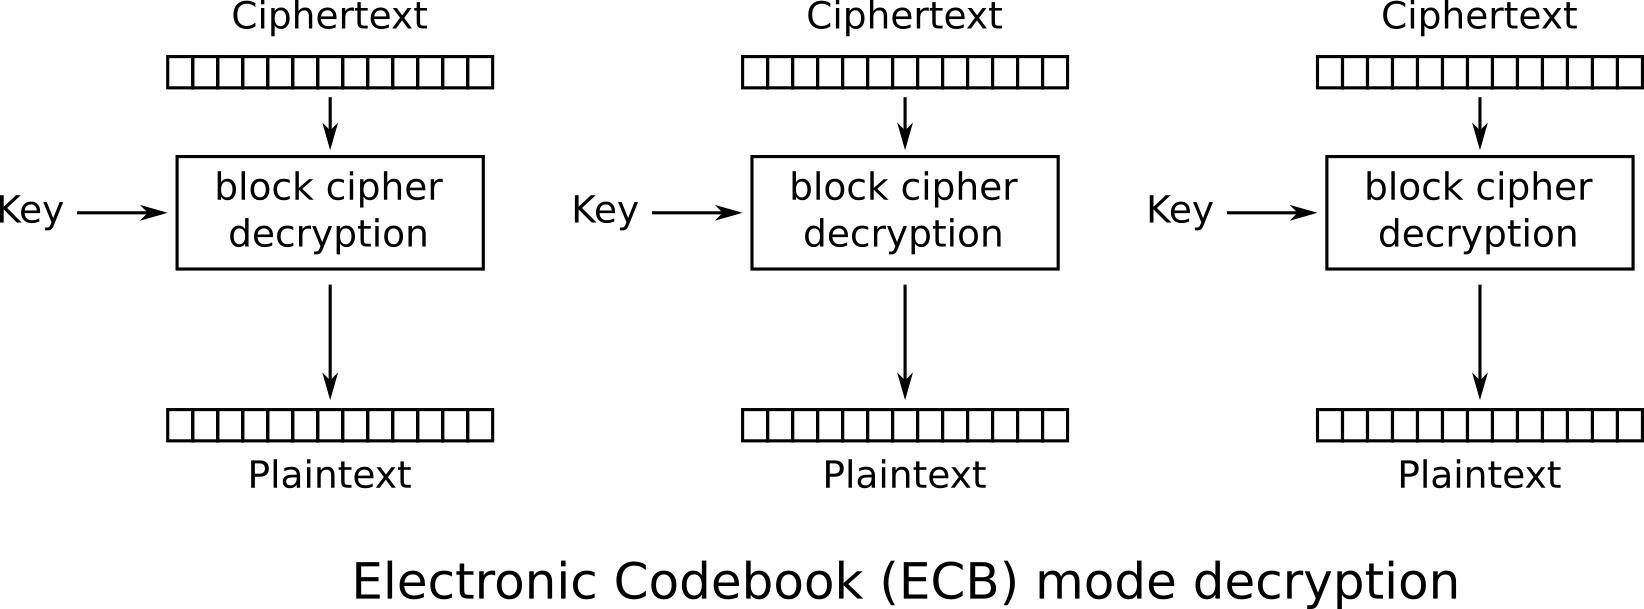
\includegraphics[scale=0.55]{./Drawings/EDIN01-Cryptography/ECB_Mode-Decryption.png}
    \caption{\nameref{subsubsec:Electronic_Codebook_Mode} Decryption Steps}
    \label{subfig:ECB_Mode_Steps_Decryption}
  \end{subfigure}
  \caption{\nameref*{subsubsec:Electronic_Codebook_Mode} Steps}
  \label{fig:Electronic_Codebook_Mode_Steps}
\end{figure}

\paragraph{Problems with \nameref*{subsubsec:Electronic_Codebook_Mode}}\label{par:Problems_Electronic_Codebook_Mode}
If 2 plaintext blocks are the same, then the 2 corresponding ciphertext blocks are \emph{also} the same.
For example,
\begin{figure}[ht!]
  \centering
  \begin{subfigure}[h!]{0.45\linewidth}
    \centering
    
\includegraphics[scale=0.50]{./Drawings/EDIN01-Cryptography/Tux.png}
    \caption{Original Plaintext}
    \label{subfig:ECB_Mode_Plaintext_Input}
  \end{subfigure}
  \begin{subfigure}[h!]{0.45\linewidth}
    \centering
    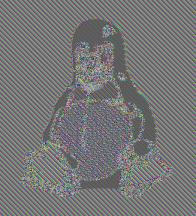
\includegraphics[scale=0.55]{./Drawings/EDIN01-Cryptography/Tux_ECB.jpg}
    \caption{ECB Mode Encrypted Plaintext}
    \label{subfig:ECB_Mode_Encrypted_Plaintext}
  \end{subfigure}
  \caption{Problem with ECB Mode}
  \label{fig:Problem_Electronic_Codebook_Mode}
\end{figure}

Notice how one could still make out the outline of the image in \Cref{subfig:ECB_Mode_Encrypted_Plaintext}.
This is undesirable, because some information is still leaked to the attacker, even after encryption.
Obviously, we need something better than ECB Mode.

\subsubsection{Cipher Block Chaining (CBC) Mode}\label{subsubsec:Cipher_Block_Chaining_Mode}
\begin{definition}[Cipher Block Chaining Mode]\label{def:Cipher_Block_Chaining_Mode}
  \emph{Cipher Block Chaining Mode} (\emph{CBC Mode}) follows a different rule.
  \begin{equation}\label{eq:Cipher_Block_Chaining_Mode_Encryption}
    Y_{i} = E_{K}(Y_{i-1} \XOR X_{i})
  \end{equation}
  where $Y_{0}$ is the \nameref{def:Initialization_Vector}.
\end{definition}

The steps required to operate a block cipher in CBC mode are illustrated in \Crefrange{subfig:CBC_Mode_Steps_Encryption}{subfig:CBC_Mode_Steps_Decryption}.
\begin{figure}[ht!]
  \centering
  \begin{subfigure}[h!]{0.45\linewidth}
    \centering
    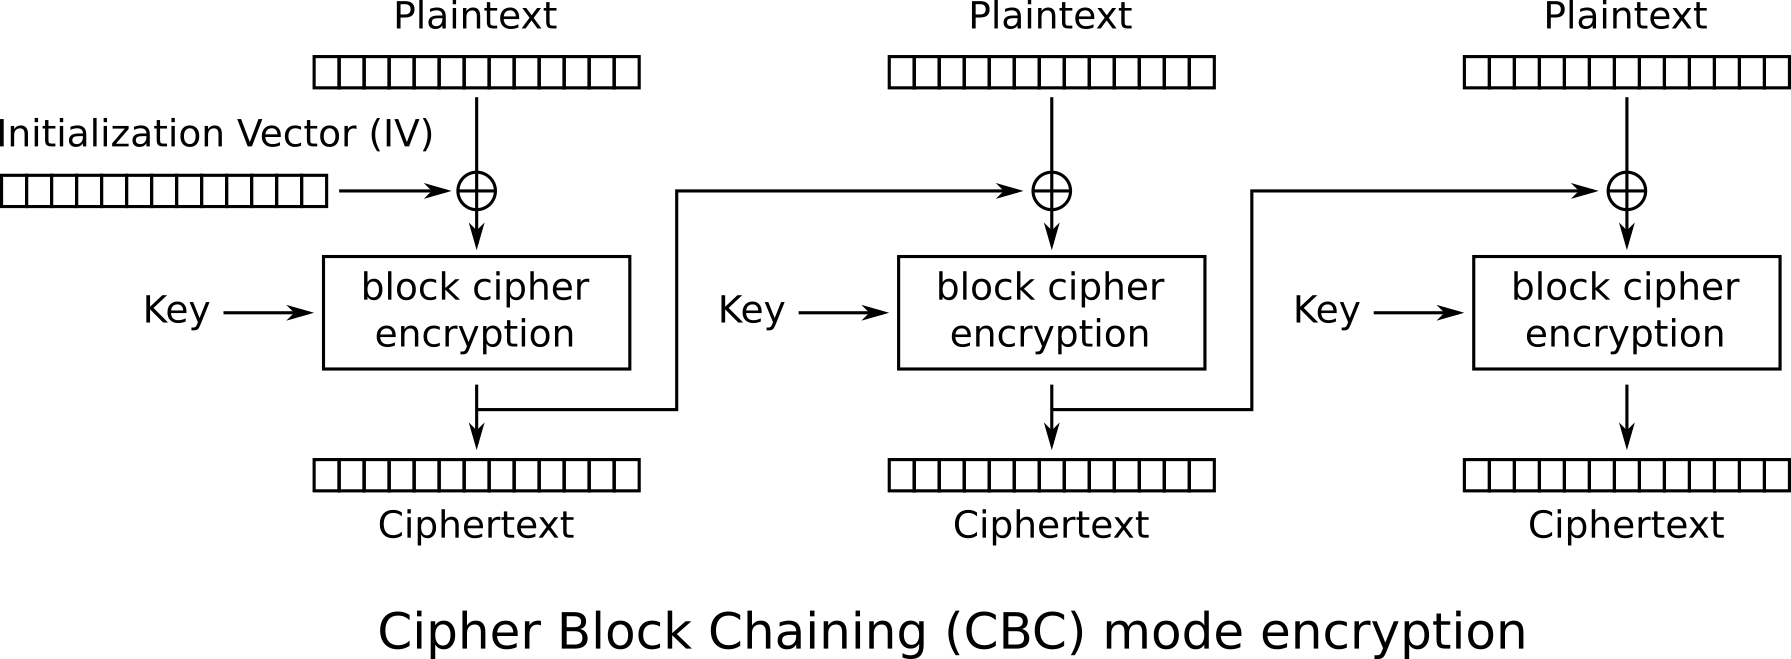
\includegraphics[scale=0.55]{./Drawings/EDIN01-Cryptography/CBC_Mode-Encryption.png}
    \caption{\nameref{def:Cipher_Block_Chaining_Mode} Encryption Steps}
    \label{subfig:CBC_Mode_Steps_Encryption}
  \end{subfigure}
  \vline{}
  \begin{subfigure}[h!]{0.45\linewidth}
    \centering
    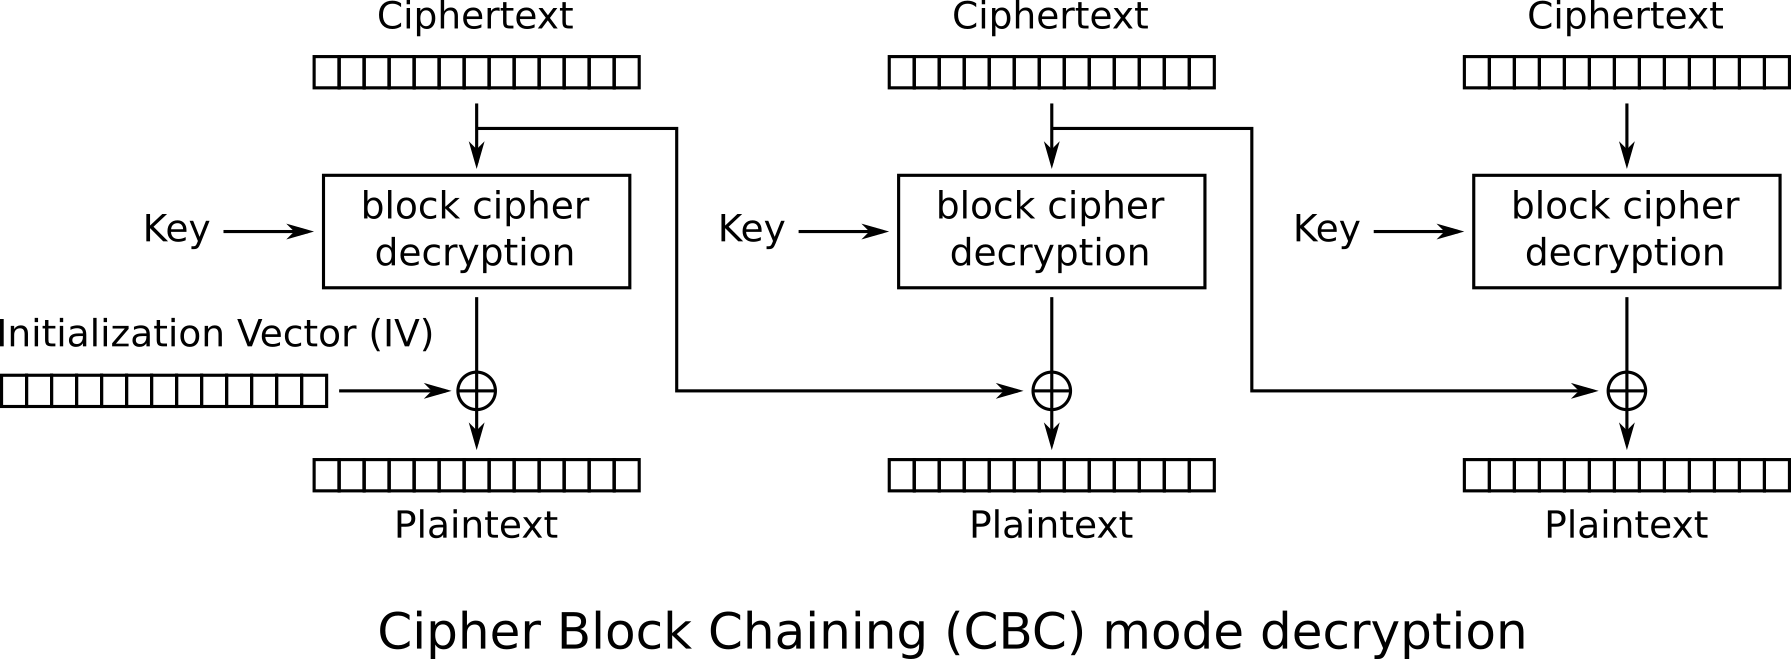
\includegraphics[scale=0.55]{./Drawings/EDIN01-Cryptography/CBC_Mode-Decryption.png}
    \caption{\nameref{def:Cipher_Block_Chaining_Mode} Decryption Steps}
    \label{subfig:CBC_Mode_Steps_Decryption}
  \end{subfigure}
  \caption{\nameref*{def:Cipher_Block_Chaining_Mode} Steps}
  \label{fig:Cipher_Block_Chaining_Mode_Steps}
\end{figure}

\subsubsection{Counter Mode}\label{subsubsec:Counter_Mode}
\begin{definition}[Counter Mode]\label{def:Counter_Mode}
  \emph{Counter Mode} is another \nameref{def:Mode_of_Operation} that actually turns our \nameref{def:Block_Cipher} into a \nameref{def:Stream_Cipher}.
  In this \nameref{def:Mode_of_Operation}, the \emph{count} of which block we are working with is encrypted.
  Then, the encrypted count is XORed with the plaintext message, to produce our ciphertext message.

  The keystream sequence is given by
  \begin{equation}\label{eq:Counter_Mode_Keystream_Sequence}
    E_{K}(0), E_{K}(1), E_{K}(2), \ldots
  \end{equation}
\end{definition}

The steps required to operate a block cipher in counter mode are illustrated in \Crefrange{subfig:Counter_Mode_Steps_Encryption}{subfig:Counter_Mode_Steps_Decryption}.
\begin{figure}[ht!]
  \centering
  \begin{subfigure}[h!]{0.45\linewidth}
    \centering
    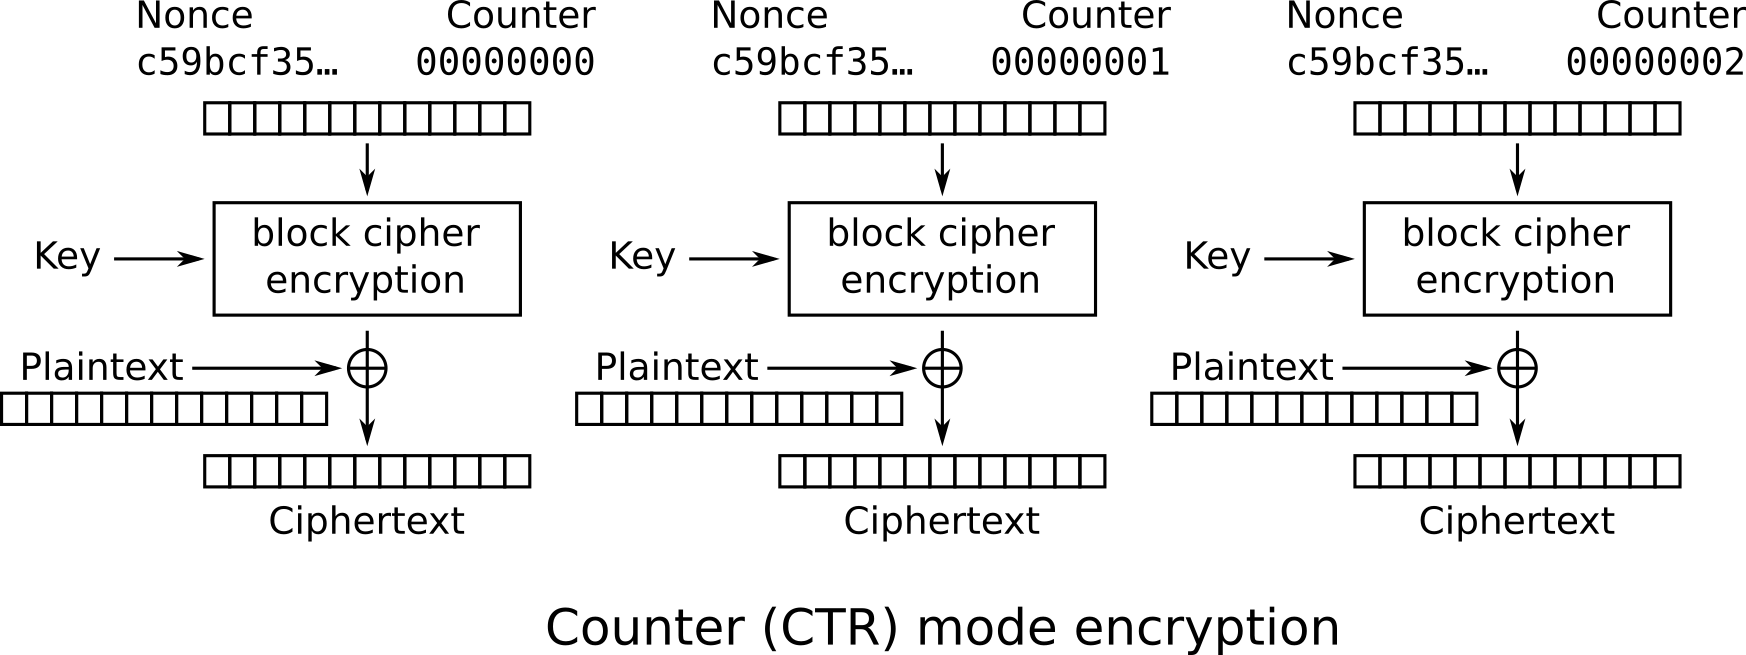
\includegraphics[scale=0.55]{./Drawings/EDIN01-Cryptography/Counter_Mode-Encryption.png}
    \caption{\nameref{def:Counter_Mode} Encryption Steps}
    \label{subfig:Counter_Mode_Steps_Encryption}
  \end{subfigure}
  \vline{}
  \begin{subfigure}[h!]{0.45\linewidth}
    \centering
    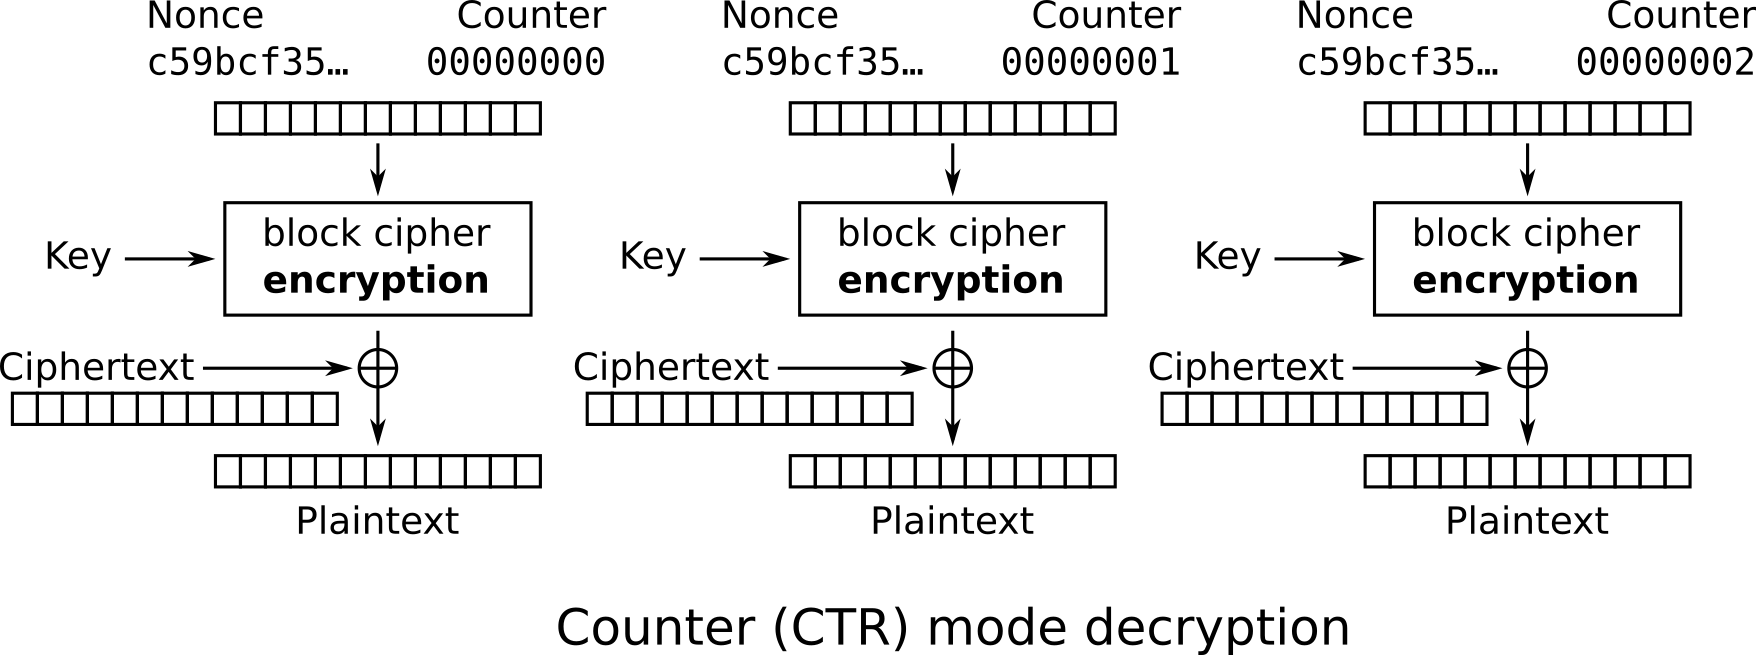
\includegraphics[scale=0.55]{./Drawings/EDIN01-Cryptography/Counter_Mode-Decryption.png}
    \caption{\nameref{def:Counter_Mode} Decryption Steps}
    \label{subfig:Counter_Mode_Steps_Decryption}
  \end{subfigure}
  \caption{\nameref*{def:Cipher_Block_Chaining_Mode} Steps}
  \label{fig:Cipher_Block_Chaining_Mode_Steps}
\end{figure}

\subsection{Advanced Encryption Scheme}\label{subsec:AES}
\textbf{TODO}
\begin{definition}[Advanced Encryption Scheme]\label{def:AES}
  \textbf{TODO}
  The \emph{Advanced Encryption Scheme} (\emph{AES}) cipher is a \nameref{def:SP_Network} \nameref{def:Block_Cipher}.
  It was originally designed to be fast in both hardware and software.
  Today, it is faster to perform these calculations in software because CPU architectures support special instructions just for these calculations.

  In AES, the block size is fixed to 128 bits.
  The key size is variable; either: 128 bits, 192 bits, or 256 bits.
  These different key sizes correspond to the the number of rounds that happen (10, 12, or 14, respectively).

  AES operates on binary matrices.
  They are $2 \times 2$ matrices where each element is a byte (8 bits).
  AES has several steps involved in it.
  \begin{enumerate}[noitemsep]
  \item The first round is always a round of \nameref{subsubsec:AES-AddRoundKey}.
  \item Then, all subsequent rounds perform \emph{one} of these actions
    \begin{enumerate}[noitemsep]
    \item \nameref{subsubsec:AES-AddRoundKey}
    \item \nameref{subsubsec:AES-SubBytes}
    \item \nameref{subsubsec:AES-ShiftRows}
    \item \nameref{subsubsec:AES-MixColumns}
      \begin{itemize}[noitemsep]
      \item This is \emph{not} run on the last round.
      \end{itemize}
    \end{enumerate}
  \end{enumerate}

  AES has been broken in practice, but not in a practical sense.
  The best known attacks were on 7 rounds for 128-bit keys, 8 rounds for 192-bit keys, and 9 rounds for 256-bit keys.
  \textbf{Side-Channel attacks are still possible (cache-timing attacks, differential fault analysis, etc.)}.

  \begin{remark}[Other Cryptographic Primitive's Reliance on \nameref*{def:AES}]\label{rmk:Other_Crypto_Primitive_Reliance_AES}
    Many other \nameref{def:Cryptographic_Primitive}s rely on the security of \nameref{def:AES}.
    This means that these derived \nameref{def:Cryptographic_Primitive}s are as secure as \nameref{def:AES}.
  \end{remark}
\end{definition}

%%% Local Variables:
%%% mode: latex
%%% TeX-master: "../EDIN01-Cryptography-Reference_Sheet"
%%% End:
